\subsection{Paquete 6: Motor de tareas domésticas y sistema de puntos}

    El paquete automatiza la asignación y supervisión de las tareas del hogar. Implementa un motor de rotación equitativa (\emph{Round-Robin}), un calendario compartido de turnos, incentivos gamificados mediante puntuaciones y una función de rescate para tareas vencidas. La figura \ref{fig:dcu_tareas} expone los siete casos de uso del subsistema (CU57 a CU63).

\begin{figure}[H]
    \centering
    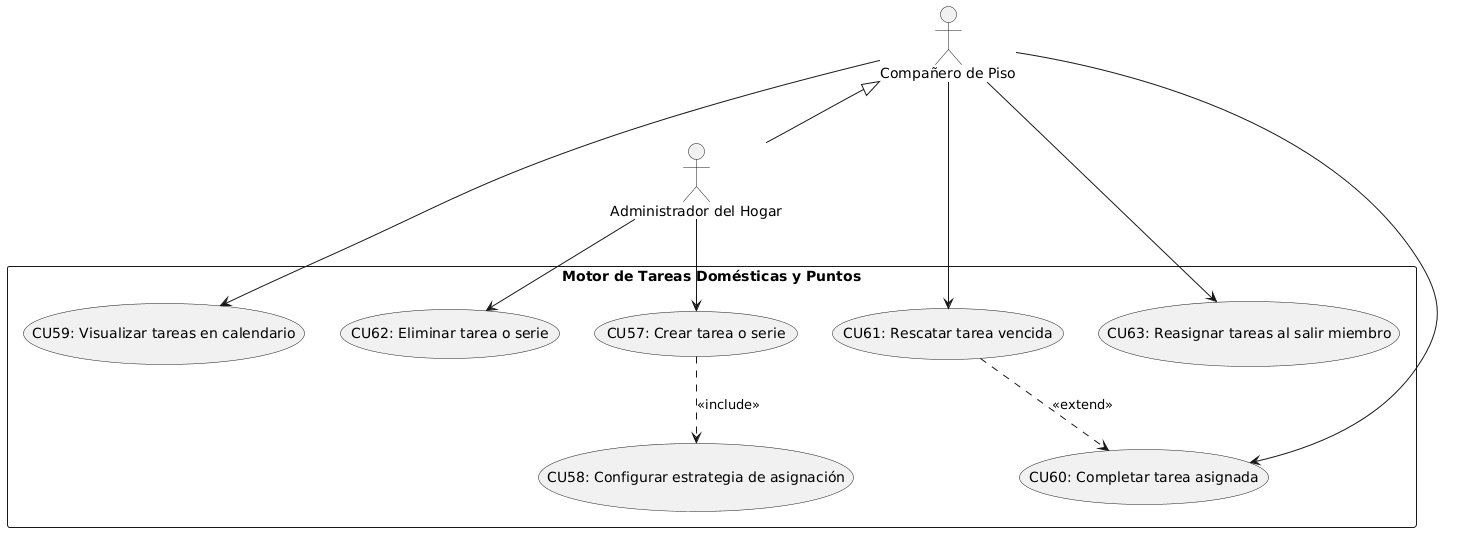
\includegraphics[width=0.78\textwidth]{AnalisisFuncional/img/dcu_tareas.png}
    \caption{Diagrama de casos de uso de tareas domésticas y puntos}
    \label{fig:dcu_tareas}
\end{figure}

    Las siguientes fichas estructuran el comportamiento de CU57 a CU63:

\begin{table}[H]
\centering
\begin{tabular}{|p{3.2cm}|p{11.3cm}|}
\hline
\textbf{Caso de Uso} & \textbf{CU57: Crear tarea única o serie recurrente} \\ \hline
\textbf{Actores} & Administrador del Hogar \\ \hline
\textbf{Descripción} & Da de alta una labor doméstica puntual o una serie periódica vinculada a un valor en puntos \\ \hline
\textbf{Precondiciones} & Ostentar el rol de administrador en el hogar correspondiente \\ \hline
\textbf{Flujo básico} & 
1. El administrador accede al planificador de tareas y pulsa sobre la opción de nueva labor. \newline
2. El administrador define el título, descripción, periodicidad, fecha límite y recompensa en puntos. \newline
3. Se invoca de forma obligatoria la configuración de la estrategia de asignación de miembros. \newline
4. El backend genera la serie o tarea única y la incorpora al calendario general del piso. \\ \hline
\end{tabular}
\caption{Especificación del caso de uso CU57}
\label{tab:cu57}
\end{table}

\begin{table}[H]
\centering
\begin{tabular}{|p{3.2cm}|p{11.3cm}|}
\hline
\textbf{Caso de Uso} & \textbf{CU58: Configurar estrategia de asignación} \\ \hline
\textbf{Actores} & Administrador del Hogar \\ \hline
\textbf{Descripción} & Determina la política de adjudicación de turnos entre fija o rotativa equitativa \\ \hline
\textbf{Precondiciones} & Estar en proceso de creación o parametrización de una labor doméstica \\ \hline
\textbf{Flujo básico} & 
1. El administrador elige si la tarea recae siempre en un miembro fijo o en una secuencia cíclica. \newline
2. En caso rotativo, el sistema ordena a los compañeros activos para repartir la carga. \newline
3. El motor de planificación almacena el orden de turnos asociado a la serie. \\ \hline
\end{tabular}
\caption{Especificación del caso de uso CU58}
\label{tab:cu58}
\end{table}

\begin{table}[H]
\centering
\begin{tabular}{|p{3.2cm}|p{11.3cm}|}
\hline
\textbf{Caso de Uso} & \textbf{CU59: Visualizar tareas en calendario y cuadrante} \\ \hline
\textbf{Actores} & Compañero de Piso \\ \hline
\textbf{Descripción} & Muestra el estado de las labores domésticas en formato de cuadrante mensual o lista diaria \\ \hline
\textbf{Precondiciones} & Formar parte activa del espacio de convivencia \\ \hline
\textbf{Flujo básico} & 
1. El compañero abre el panel de tareas domésticas en la interfaz. \newline
2. El sistema recupera las tareas programadas con su estado (pendiente, completada o vencida). \newline
3. La interfaz renderiza las labores diferenciando a los asignatarios por su código de color. \\ \hline
\end{tabular}
\caption{Especificación del caso de uso CU59}
\label{tab:cu59}
\end{table}

\begin{table}[H]
\centering
\begin{tabular}{|p{3.2cm}|p{11.3cm}|}
\hline
\textbf{Caso de Uso} & \textbf{CU60: Completar tarea asignada} \\ \hline
\textbf{Actores} & Compañero de Piso \\ \hline
\textbf{Descripción} & Marca una labor asignada como finalizada sumando los puntos previstos al perfil \\ \hline
\textbf{Precondiciones} & Que la tarea figure asignada al usuario y no se encuentre ya convalidada \\ \hline
\textbf{Flujo básico} & 
1. El compañero selecciona su tarea pendiente en el cuadrante y confirma su realización. \newline
2. El backend marca la labor en estado completada y registra la marca de tiempo de cierre. \newline
3. El sistema añade los puntos de recompensa al balance de gamificación del usuario. \newline
4. Si la tarea formaba parte de una serie rotativa, el sistema planifica la siguiente iteración. \\ \hline
\end{tabular}
\caption{Especificación del caso de uso CU60}
\label{tab:cu60}
\end{table}

\begin{table}[H]
\centering
\begin{tabular}{|p{3.2cm}|p{11.3cm}|}
\hline
\textbf{Caso de Uso} & \textbf{CU61: Rescatar tarea vencida de otro miembro} \\ \hline
\textbf{Actores} & Compañero de Piso \\ \hline
\textbf{Descripción} & Asume y completa una labor fuera de plazo no realizada por otro compañero sumando puntos extra \\ \hline
\textbf{Precondiciones} & Que la labor se encuentre formalmente vencida y asignada originalmente a otro compañero \\ \hline
\textbf{Flujo básico} & 
1. El compañero localiza una tarea expirada en el tablón común y activa la opción de rescate. \newline
2. El sistema transfiere de forma transitoria la asignación de la labor al nuevo usuario. \newline
3. Se invoca de forma extendida el caso de uso de completar tarea asignada. \newline
4. El sistema asigna la bonificación de puntos al rescatador y emite notificación al piso. \\ \hline
\end{tabular}
\caption{Especificación del caso de uso CU61}
\label{tab:cu61}
\end{table}

\begin{table}[H]
\centering
\begin{tabular}{|p{3.2cm}|p{11.3cm}|}
\hline
\textbf{Caso de Uso} & \textbf{CU62: Eliminar tarea o serie recurrente} \\ \hline
\textbf{Actores} & Administrador del Hogar \\ \hline
\textbf{Descripción} & Da de baja una tarea programada o cancela de manera definitiva una serie recurrente \\ \hline
\textbf{Precondiciones} & Poseer privilegios de administración en el espacio doméstico \\ \hline
\textbf{Flujo básico} & 
1. El administrador selecciona la labor a suprimir y elige entre borrar la instancia o la serie entera. \newline
2. El sistema solicita confirmación advirtiendo sobre las asignaciones futuras afectadas. \newline
3. El backend purga los registros planificados y recalcula el calendario del hogar. \\ \hline
\end{tabular}
\caption{Especificación del caso de uso CU62}
\label{tab:cu62}
\end{table}

\begin{table}[H]
\centering
\begin{tabular}{|p{3.2cm}|p{11.3cm}|}
\hline
\textbf{Caso de Uso} & \textbf{CU63: Reasignar tareas al salir un miembro} \\ \hline
\textbf{Actores} & Compañero de Piso, Administrador del Hogar \\ \hline
\textbf{Descripción} & Redistribuye automáticamente las labores que estaban asignadas a un miembro saliente \\ \hline
\textbf{Precondiciones} & Que un miembro abandone el piso o sea expulsado formalmente \\ \hline
\textbf{Flujo básico} & 
1. El sistema intercepta el proceso de desvinculación formal de un integrante. \newline
2. El backend audita todas las tareas pendientes o futuras asociadas al usuario saliente. \newline
3. El motor de rotación redistribuye las responsabilidades entre los miembros restantes. \newline
4. El sistema notifica la actualización del cuadrante a los compañeros activos. \\ \hline
\end{tabular}
\caption{Especificación del caso de uso CU63}
\label{tab:cu63}
\end{table}